\section{Обзор существующих моделей}
\label{sec:Chapter2} \index{Chapter2}

\subsection{Модели для распознавания ключевых точек на теле человека}

В данном разделе мы рассмотрим 5-6 различных моделей. В главе \ref{sec:Chapter4} мы выберем 4 наиболее удобные в использовании и в обучении и проведем эксперимент по оценке данных моделей.

Так же хочется сказать, что, помимо приведенных, есть множество моделей от одиночных авторов, не объединенных в лаборатории (ССЫЛКИ). Они в основном брали какую-то из представленных моделей и проводили небольшое улучшение.

А теперь перейдем к моделям.

\subsubsection{BlazePose}

MediaPipe является одним из проектов компании GOOGLE и в своей работе решает задачи компьютерного зрения. В нем уже были представлены модели для распознавания лица (Face Detection) и его поверхности (Face Mesh), ладоней (Hands), объектов (Object Detection и Objectron) и другие \cite{mediapipe}. Для нас же интересна задача поиска ключевых точек, которую и решает модель BlazePose \cite{BlazePose}. На момент исследования модель умеет отслеживать движения человека на видеофрагменте и строить покадровую маску человека.

Для предложенной модели была создана топология, которая представляет собой суперпозицию топологии COCO и двух других топологий, уже использовавшихся в других подпроектах MediaPipe. Об этом более подробно написано в \autoref{subsec:Theory of keypoint detection}.

\hfill \break
В BlazePose используется top-down подход оценки позы человека. Сначала запускается Pose Detector (см \autoref{fig:mp_model_structure}), который возвращает координаты интересующей нас области (region-of-interest или ROI). Алгоритм используем расширение модели BlazeFace для определения наличия человека в кадре. Поэтому данная модель чувствительна к видимости головы, лица в частности, на фотографии. Взяв идею витрувианского человека Леонардо Да Винчи, исследователям понадобилось ещё две точки для точной локализации человека на изображении.

\begin{figure}[h]
	\centering
	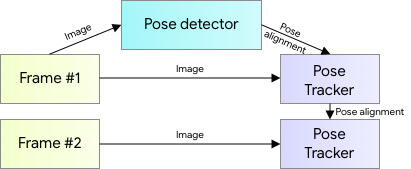
\includegraphics[width=\textwidth * 4 / 5]{./images/MPPose/Model_structure.jpg}
	\caption{Структура модели BlazePose для работы в реальном времени.\\ \href{https://1.bp.blogspot.com/-J66lTDBjlgw/XzVwzgeQJ7I/AAAAAAAAGYM/WBIhbOqzi4ICUswEOHv8r7ItJIOJgL9iwCLcBGAsYHQ/s411/image11.jpg}{Оригинальное изображение}}
	\label{fig:mp_model_structure}
\end{figure}

Следующим шагом Pose Tracker производит локализацию каждой точки в заданной ROI. Данное действие производится путем комбинированной обработки тепловой карты и данных о смещении с использованием регрессионной модели (см \autoref{fig:mp_architecture}). ВОЗМОЖНО СТОИТ ПОЧИТАТЬ ПРО ТАКУЮ ОБРАБОТКУ И ПОПОДРОБНЕЕ ЕЕ ОПИСАТЬ.

\begin{figure}[h]
	\centering
	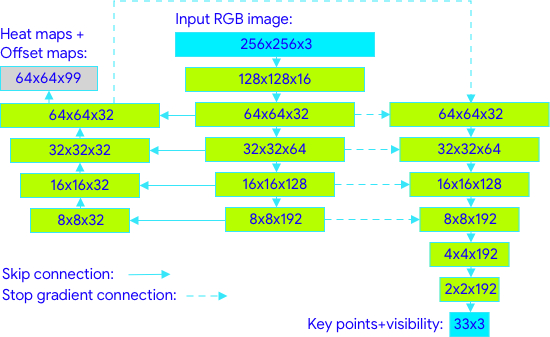
\includegraphics[width=\textwidth * 4 / 5]{./images/MPPose/architecture.jpg}
	\caption{Архитектура модели Pose Tracker.\\ \href{https://1.bp.blogspot.com/-XxKesnBALGM/XzVxSKZNWZI/AAAAAAAAGYc/WOt31icjp_YyjMxz06RSEwTi9K3qviFxwCLcBGAsYHQ/s550/image9.jpg}{Оригинальное изображение}}
	\label{fig:mp_architecture}
\end{figure}

Как можно заметить из \autoref{fig:mp_model_structure}, при аналитике видеофрагмента Pose Detector используется только на первом кадре, ведь позже данные об интересующей нас области передаются от кадра к кадру. Это упрощает вычисления и позволяет ускорить работу модели в реальном времени.

Развитием данной моели есть ее полное объединение с моделями BlazeFace и BlazeHand в модель Holistic \cite{Holistic}. Она рассматривает намного большее количество точек на лице и ладонях. НАПИСАТЬ ПРО ЕЕ ПРИМЕНЕНИЕ...


\subsubsection{MoveNet.SinglePose}

SinglePose создана для работы в веб-интерфейсах или на мобильных устройствах в режиме реального времени. Модель представлена в двух спецификациях: lightning и thunder. Первая является менее требовательной в плане мощностей и вычислений и способна обрабатывать до 50 кадров в секунду. В то же время, по заверениям создателей, вторая модель имеет большие запросы по ресурсам, но дает лучшую точность распознавания, правда со скоростью до 30 кадров в секунду.

За расположение ключевых точек выбрана классическая топология COCO. Поэтому возвращает модель координаты 17 точек, которые нормированы на размер изображения (лежат в отрезке [0, 1]).

\hfill \break
Представленная модель реализована на архитектуре MobileNetV2 \cite{mobilenetv2}. СЛОЖНАЯ АРХИТЕКТУРА. НЕОБХОДИМО ПРО НЕЕ ПРОЧИТАТЬ, А ПОТОМ УЖЕ ДОПИСАТЬ ДАННЫЙ РАЗДЕЛ.

Также существует развитие проекта MoveNet в MoveNet.MultiPose для распознавания сразу нескольких людей на изображении. Усовершенствованная модель также представлена в двух вариациях. В данной работе много персональное распознавание позы не исследовалось.

\subsubsection{OpenPose}

Проект CMU-Perceptual-Computing-Lab. В лаборатории есть множество моделей для работы отдельно с лицом, руками или что-то подобное модели Holistic от MediaPipe.

В данной модели используется топология, похожая на топологию Halpe, рассмотренную в \autoref{subsec:Theory of keypoint detection}. Рассматриваются 25 точек на теле человека. Особенностью топологии является определение положения стоп за счет детекции 3 точек на каждой.

\hfill \break
АРХИТЕКТУУУУУУУУУУУУУУРА


\subsubsection{MMPose}

Азиаты

\subsubsection{AlphaPose}

Азиаты?

\subsubsection{Detectron2}

Работает не очень приятно, но как бы она есть и то ладно. Может обойдемся без данной модели?

\subsubsection{DeepPose}

Является очень старым решением, но про него нельзя было не рассказать.


\subsection{Модели для классификации позы человека}

В данном разделе мы рассмотрим 4 различных моделей. Позже выберем 3 наиболее удобные в использовании и в обучении и проведем эксперимент по оценке данных моделей.

\subsubsection{MMaction2 by OpenMMlab}

Что-то сложное...

\subsubsection{BlazePose by MediaPipe}

Просто накинули сверху предыдущей модели kNN.

\subsubsection{mmakos}

Чувак взял OpenPose и добавил классификатор.

\subsubsection{HPC}

Уже и не помню про что тут...

\newpage